%! TEX root = ./main.tex

\section{Implementation of Decision Model}

Next, we take a man-made experimental forest in Qingping National Forest Farm in Hunan province as an example(Figure 4). We substitute the forest data\cite{Hdata,TaiwaniaDensity,ToonaDensity} into the above model to investigate the best management strategies.

\begin{figure}[htp]
    \centering
    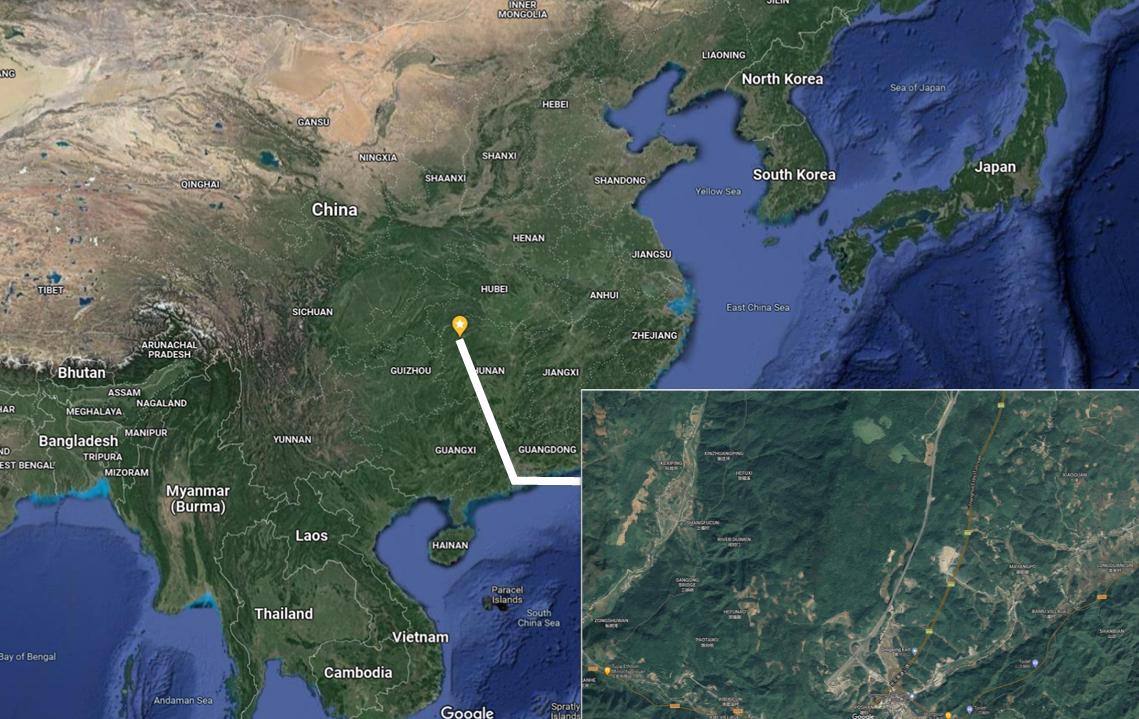
\includegraphics[width=15cm]{figs/map.png}
    \caption{Location of Qingping State-owned Forest Farm, Hunan Province, China.}
    \label{fig:my_label}
\end{figure}

\subsection{The matrix of management strategies}
By setting the 0 and 1 within the scope of different deforestation (0,0.01,0.02,0.03,0.05,0.1,0.3,0.5,1) and the different product management strategies (two extreme), get 2 x 9 matrix management plan. This strategy matrix will contain maximum and minimum values on each evaluation indicator.

We take the maximum value of the weighted sum of all factors as the objective function, realize the model solution through MATLAB programming, and get the best management  strategies. The specific process is as follows.

\subsection{Basic validation of the model}

First, We verified the relationship between total carbon sequestration and forest products and forest carbon sequestration:
$$
C(t)=\sum_{i,j}CT_{i,j}(t)+\sum_{i,j}CP_{i,j}(t)
$$

The specific case ($p_i$ =0.75, product strategy 1) is shown in figure 5. The curve relations in the other 28 cases are the same, which will not be shown in this paper.

\subsection{Management strategy}

\textbf{The management strategy} is divided into two parts: logging strategy and production strategy.

\subsubsection{Logging strategy}

Suppose the area of the three kinds of forest is 10hm$^2$. The total area of the forest farm is 30hm$^2$, and the sum of the three kinds of trees is known, that is, the southern jujube, Taiwan fir and Chinese toona. The oldest Chinese date is 35 years old, and Taiwan fir and Chinese toona are 40 years old (T$_i$). No logging is known to have taken place in these years. We get the following results:……

As a rule of thumb, we default $P_1$=25,$P_2$=50,$P_3$=38 (unit=year).

In terms of the choice of logging plan, we set different $p_i$ and obtained the curve of carbon sequestration as Figure $6$.
\begin{figure}[htbp]
\centering
\begin{minipage}[t]{0.48\textwidth}
\centering
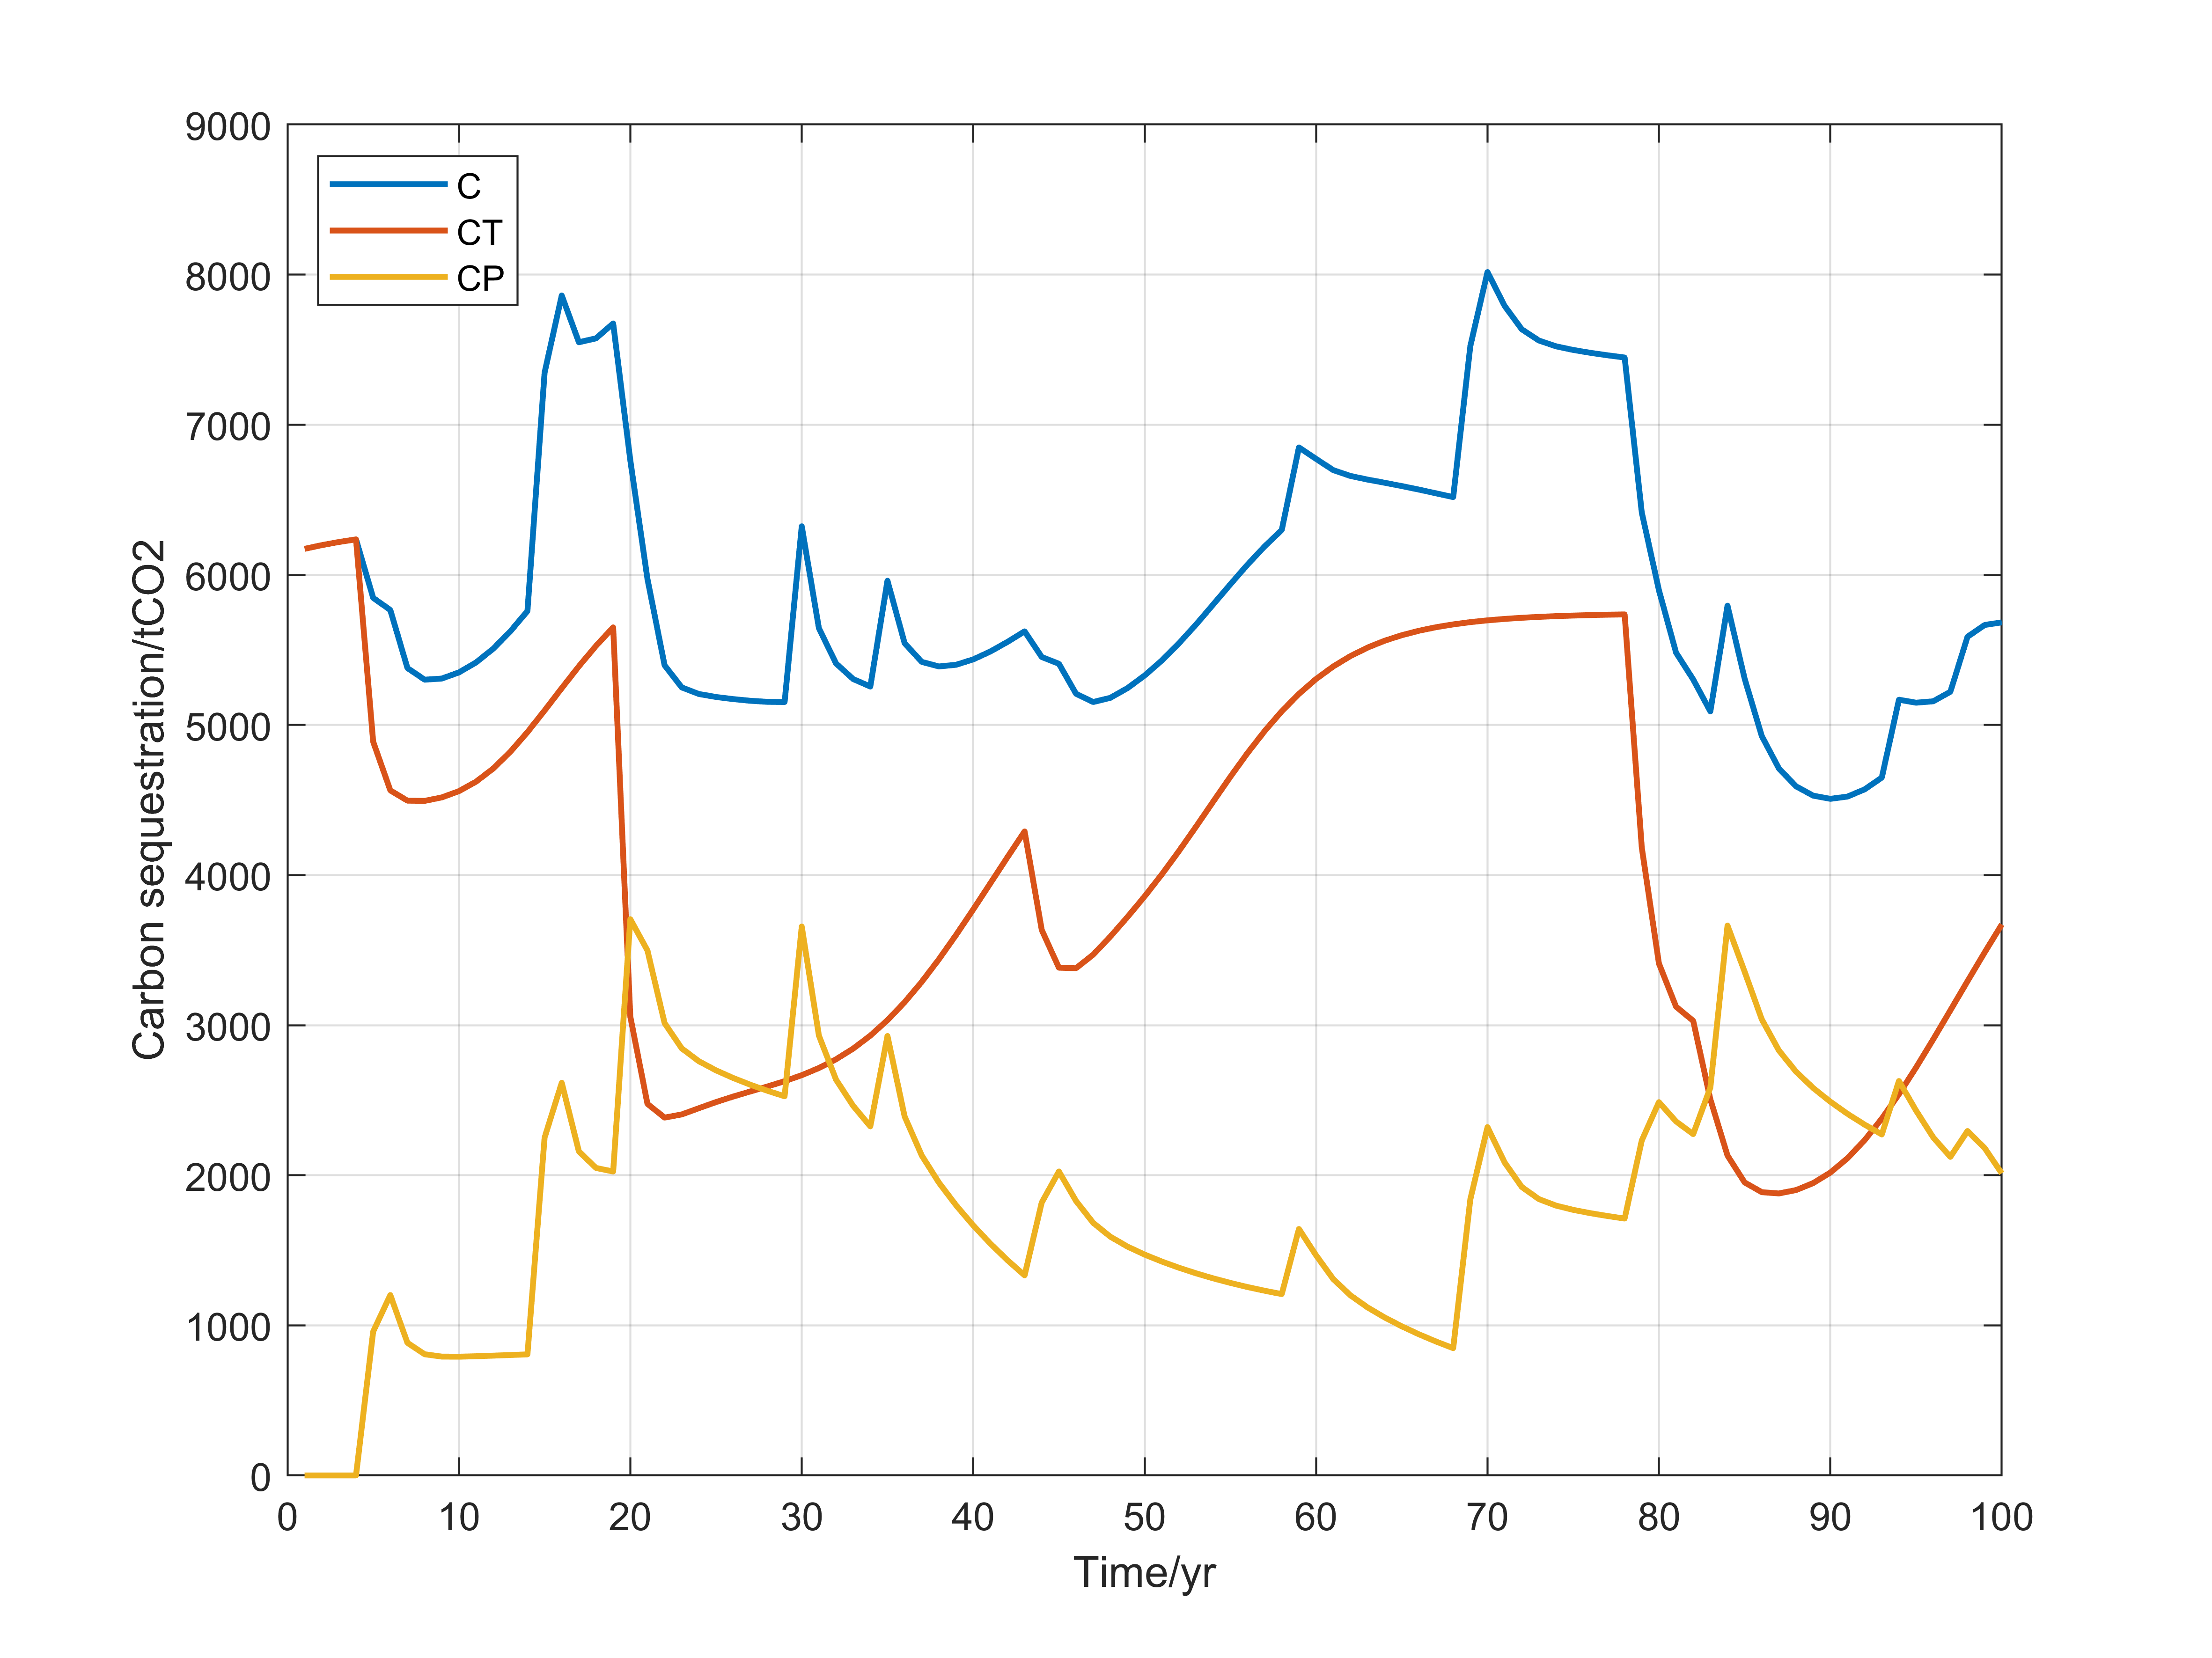
\includegraphics[width=6cm]{figs/CS.png}
\caption{Carbon sequestration under specific conditions.}
\end{minipage}
\begin{minipage}[t]{0.48\textwidth}
\centering
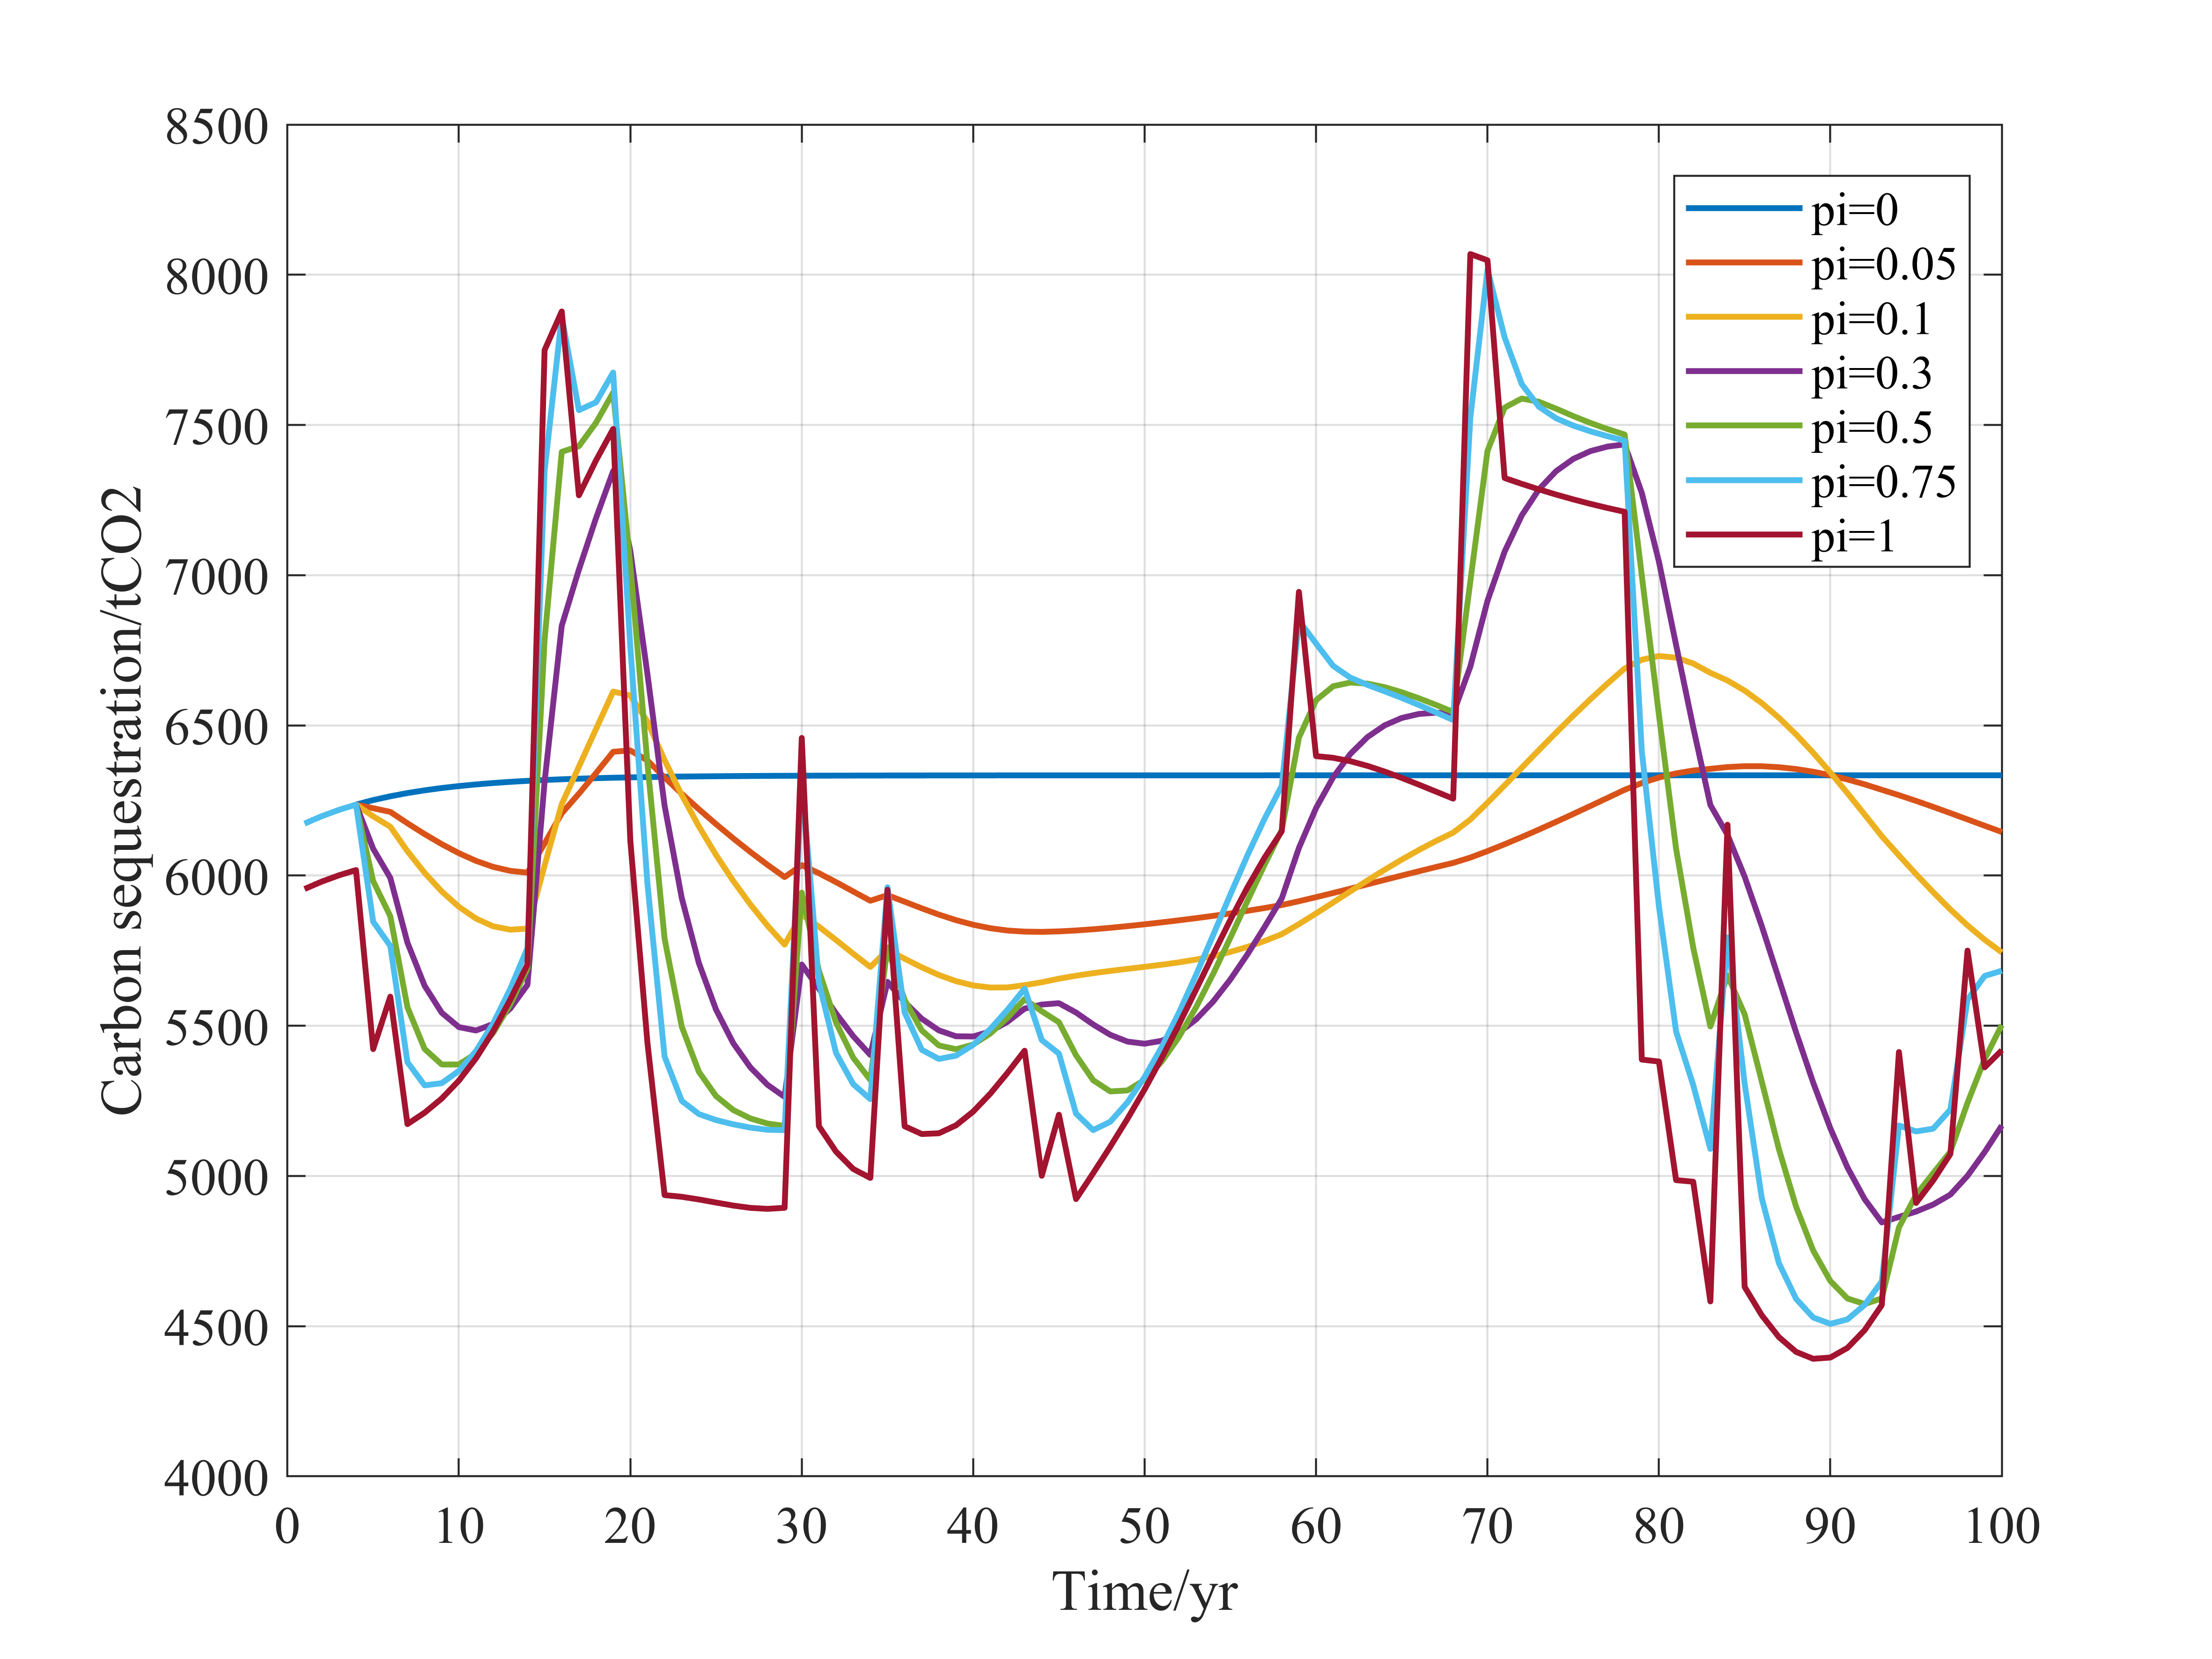
\includegraphics[width=6cm]{figs/pi_s.png}
\caption{Carbon sequestration performance of management strategies at different logging rates.}
\end{minipage}
\end{figure}

According to the results, higher carbon sequestration can be achieved when $p_i$ =0.01.

\subsubsection{Production strategy}

In terms of production strategy selection, we compared and calculated two extreme strategies:

1.$\left(\alpha_{i}, \beta_{i}, \gamma_{i}\right)=\left(0.8 \mu_{i}, 0.2 \mu_{i}+\eta_{i}, 0\right)$

2.$\left(\alpha_{i}, \beta_{i}, \gamma_{i}\right)=\left(0, \mu_{i}, \eta_{i}\right)$

As shown in Figure $7$, strategy 1 performs better in the model and can achieve higher carbon sequestration.
\begin{figure}[htbp]
\centering
\begin{minipage}[t]{0.48\textwidth}
\centering
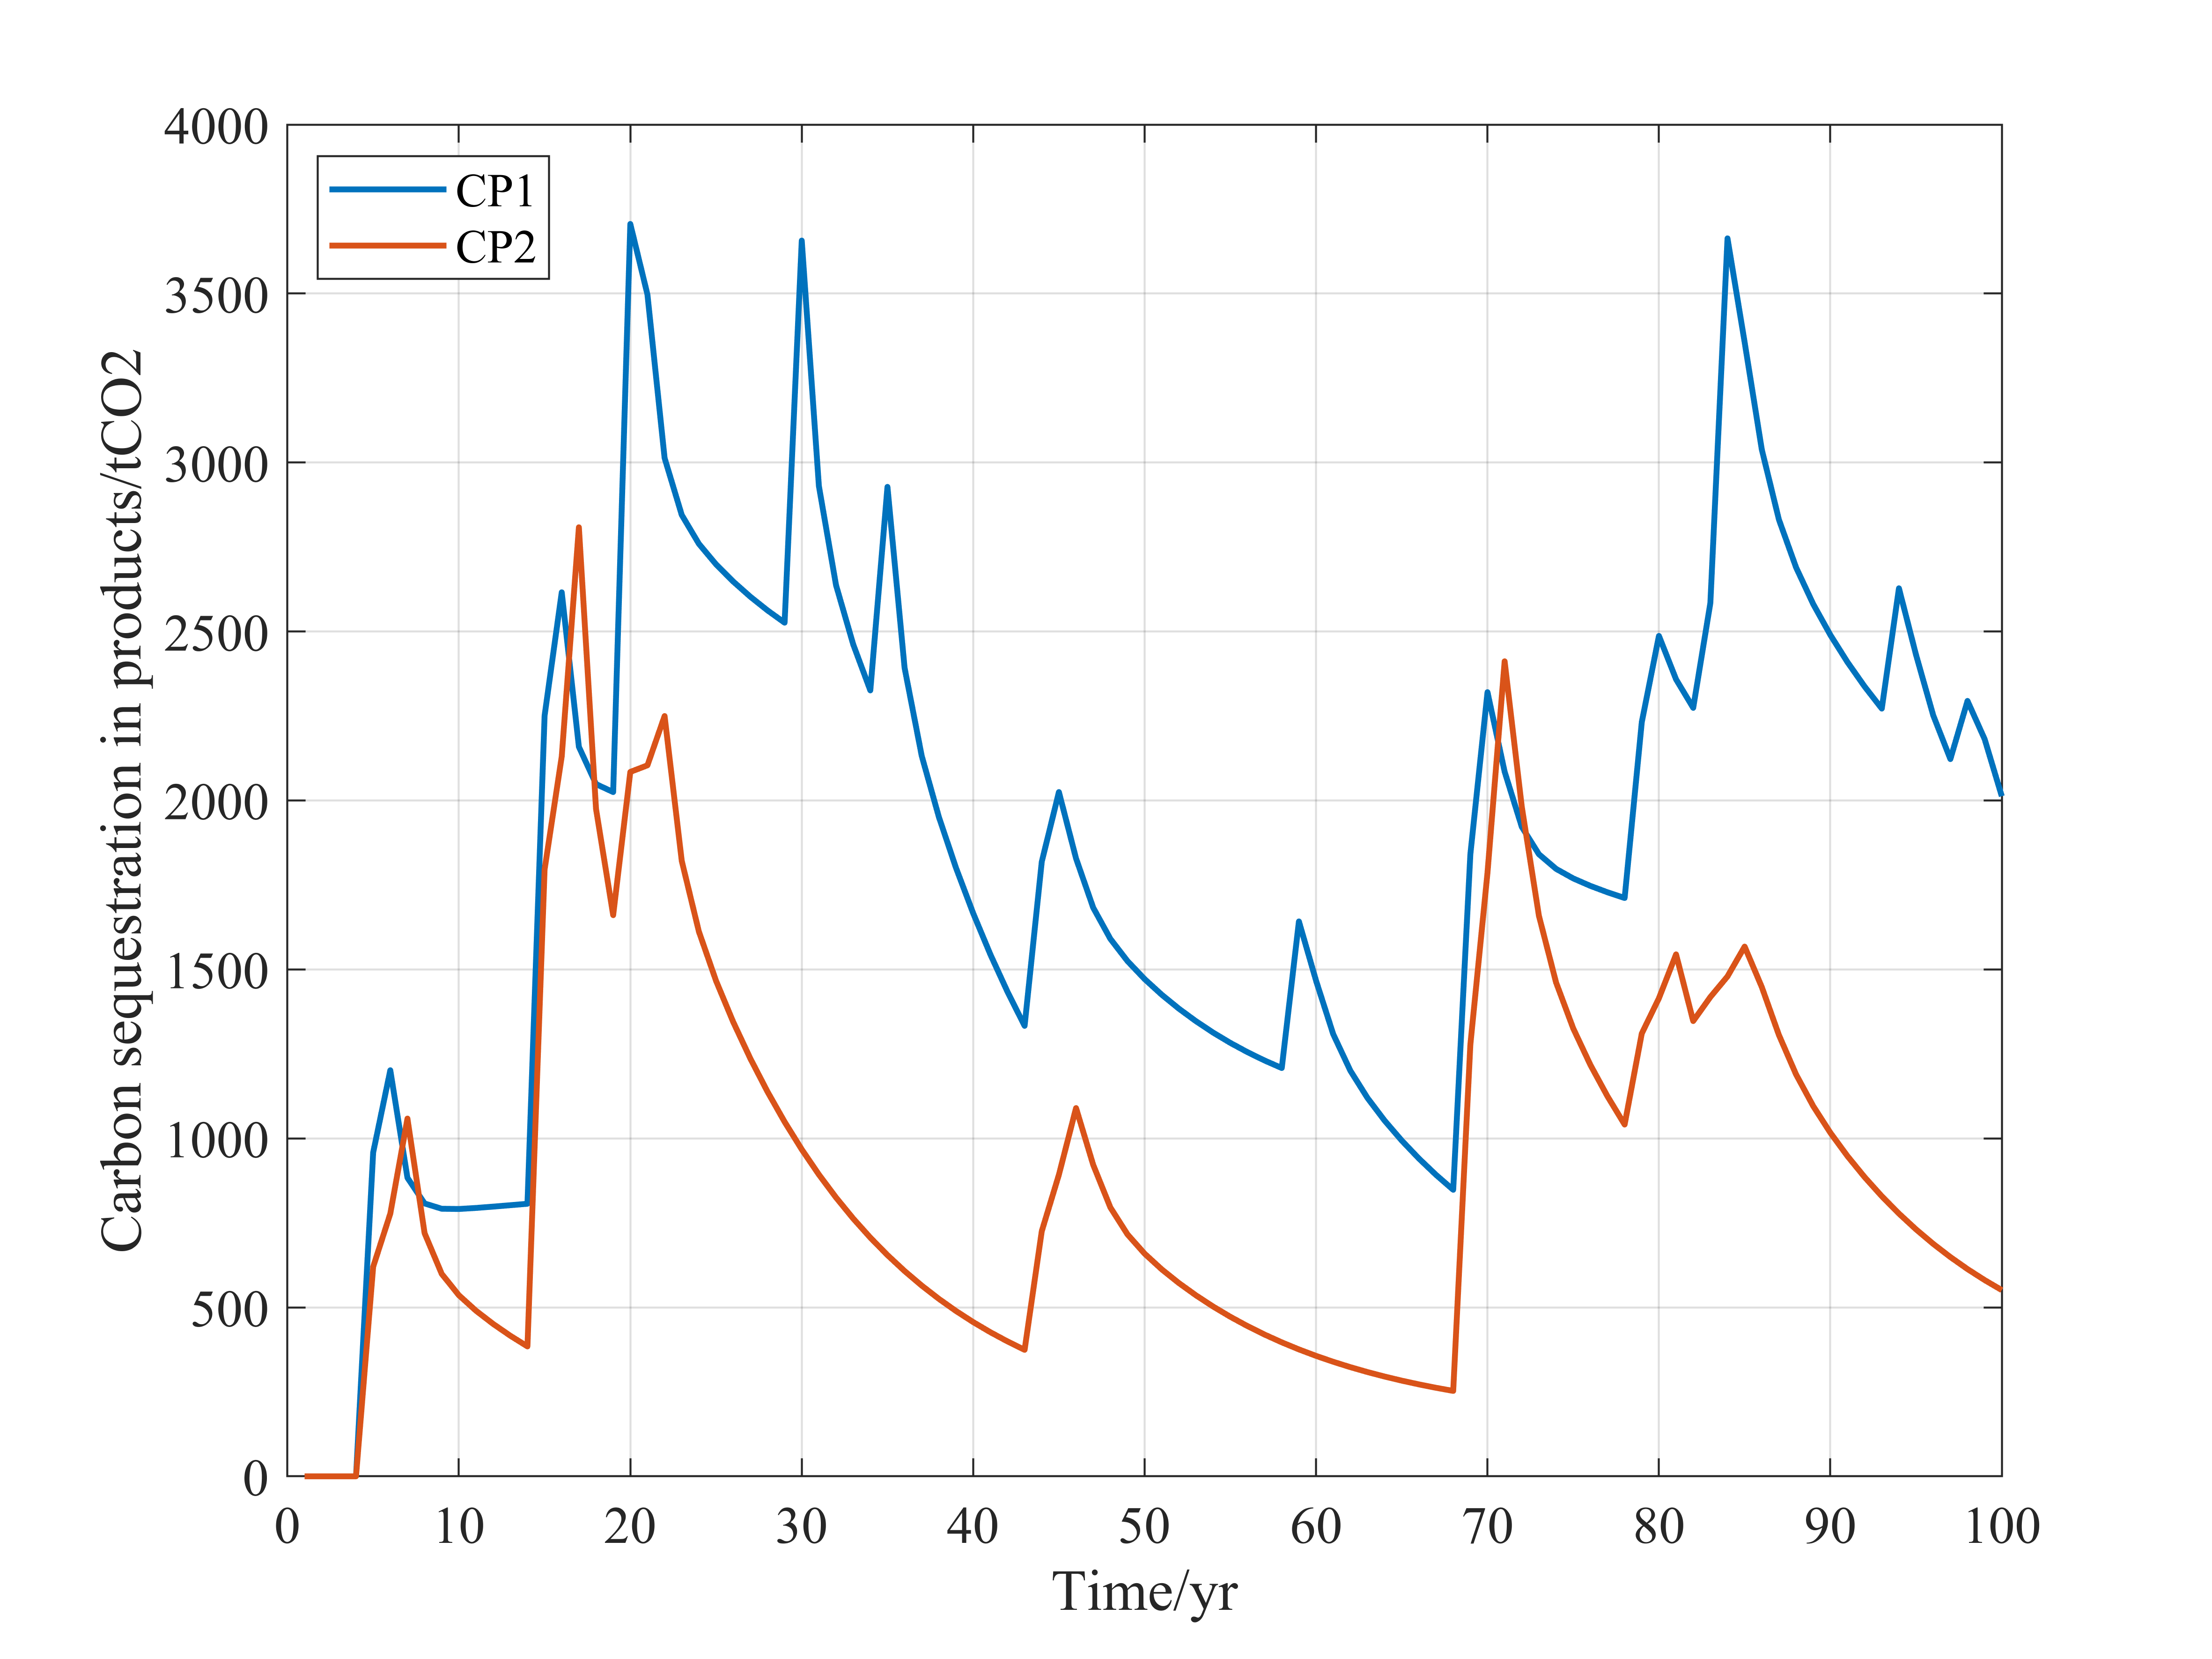
\includegraphics[width=6cm]{figs/Product_S.png}
\caption{Two extremes of product strategy choice.}
\end{minipage}
\begin{minipage}[t]{0.48\textwidth}
\centering
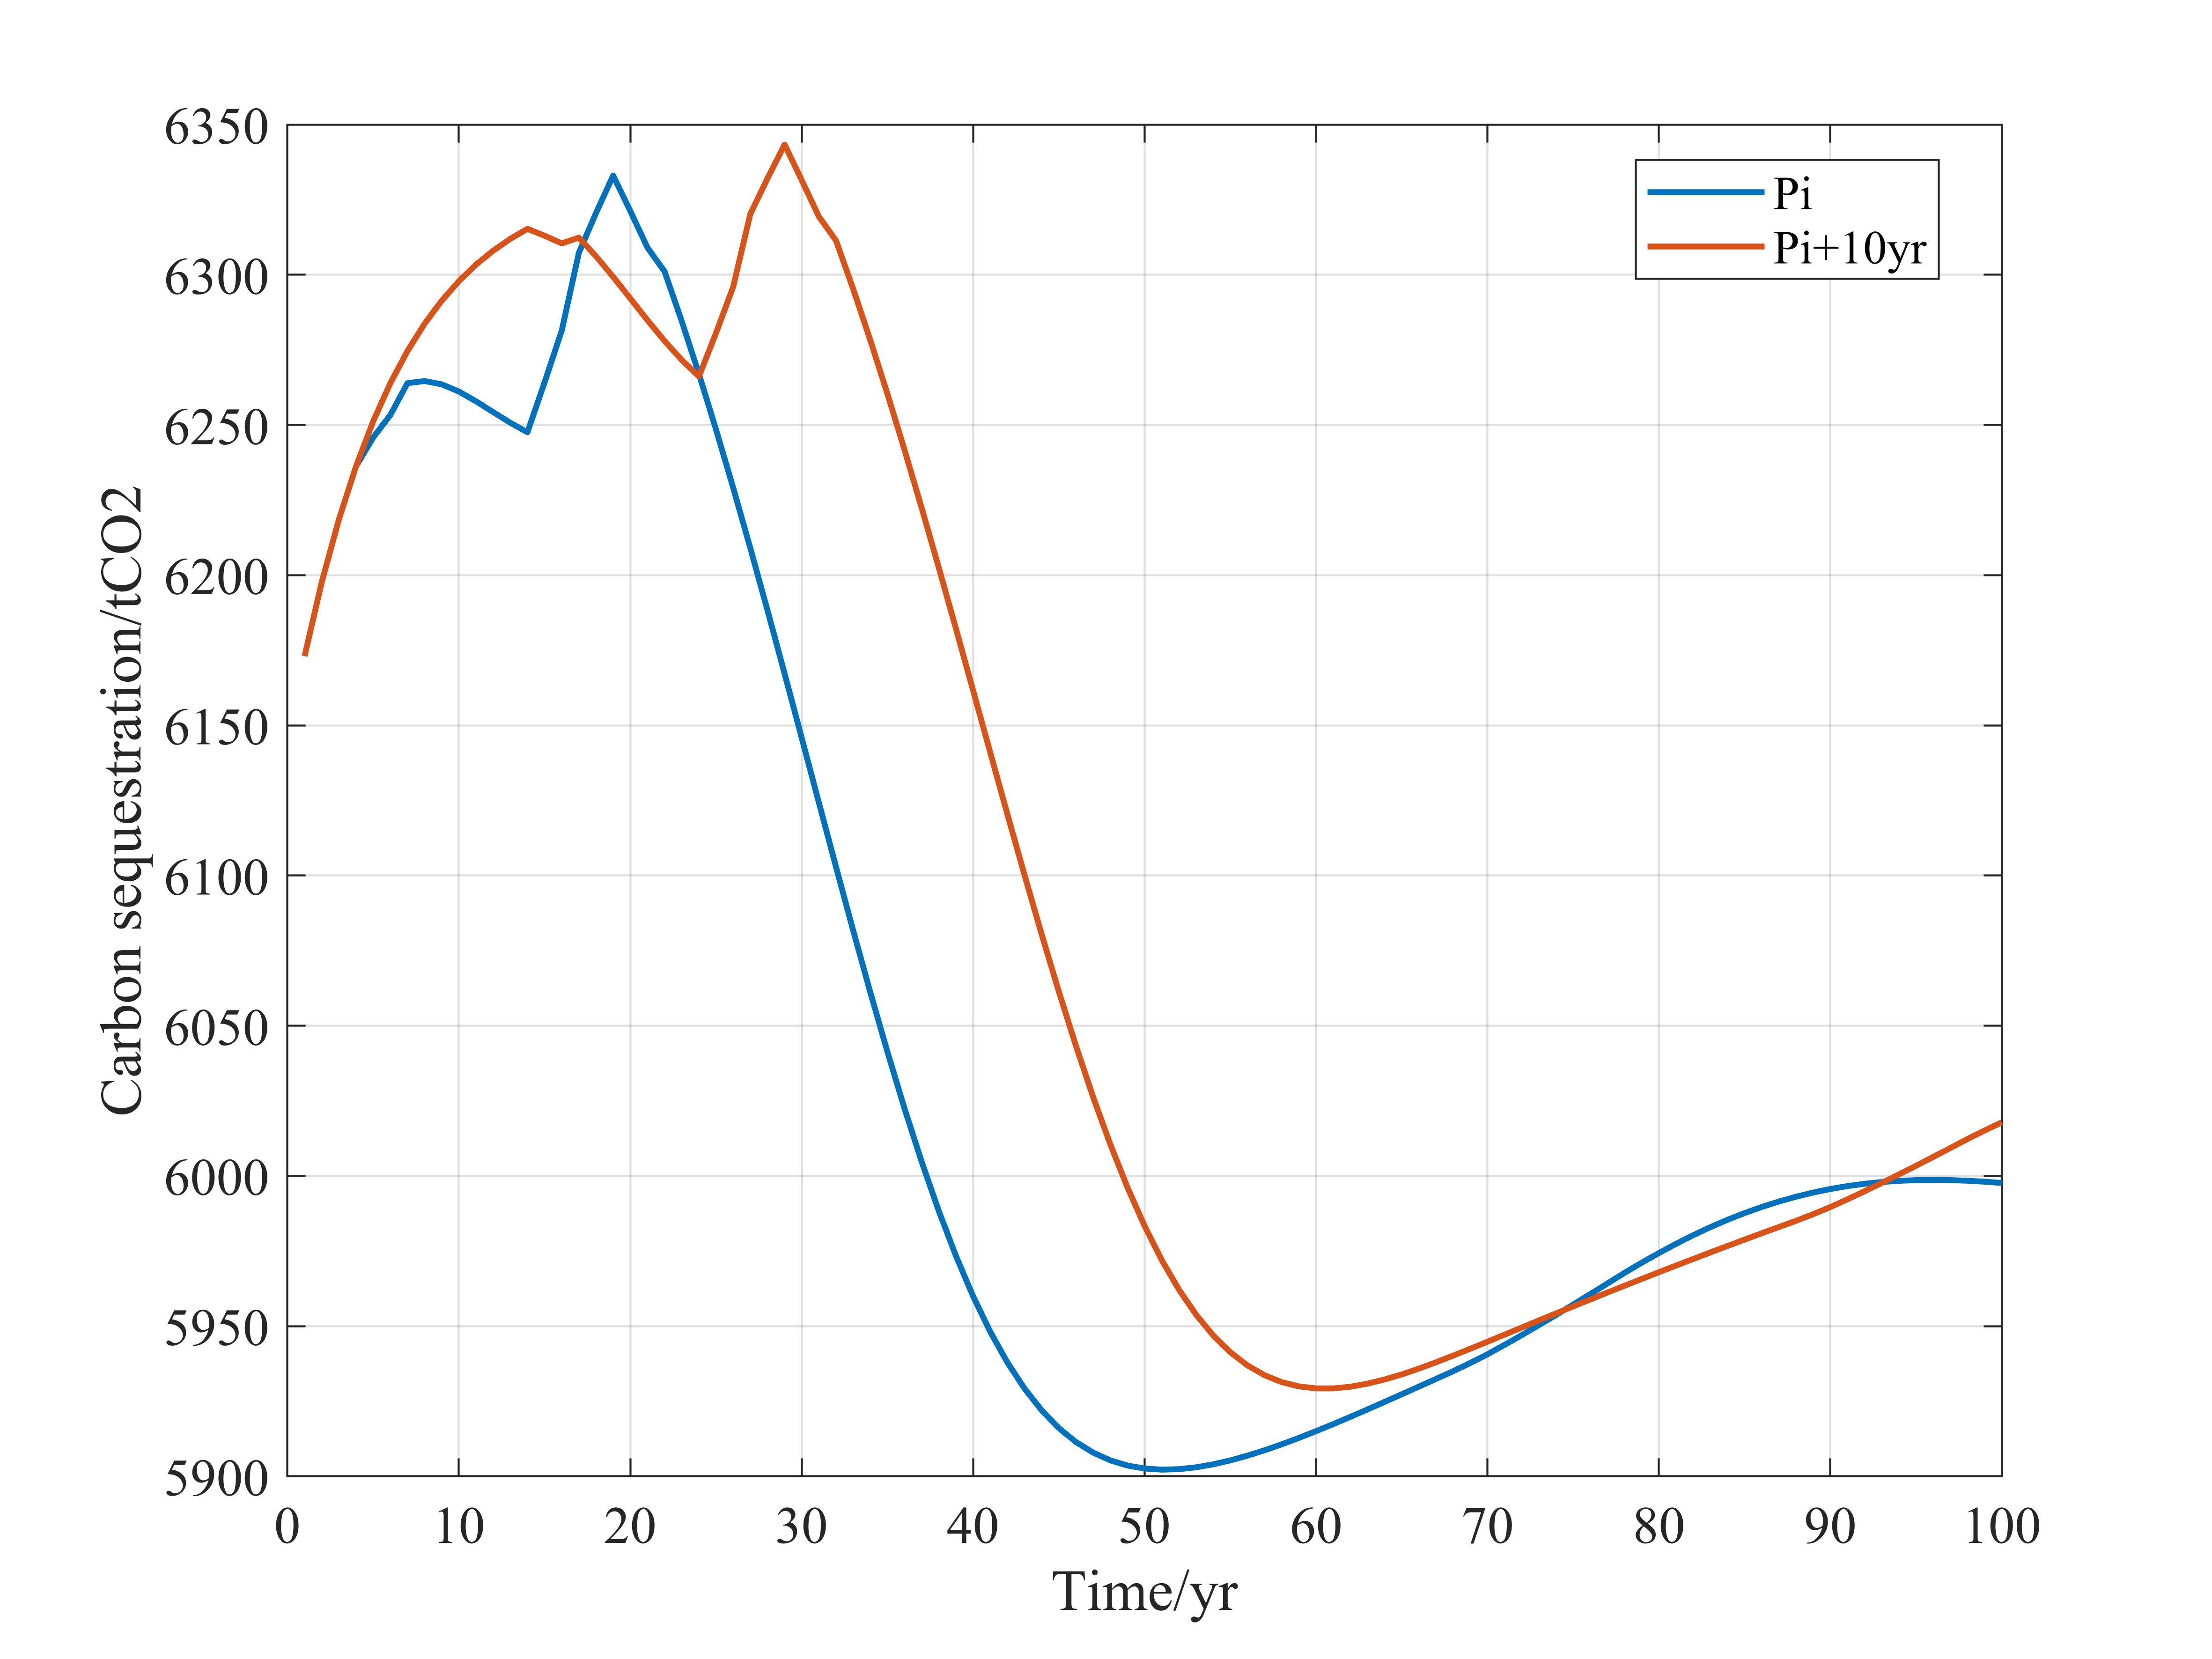
\includegraphics[width=6cm]{figs/Score.png}
\caption{Carbon sequestration of the best management strategy before and after the change of logging period.}
\end{minipage}
\end{figure}

The above analyses lead us to \textbf{the best optimal forest management strategy of pi=0.01 and strategy 2.}

\subsection{Carbon sequestration under optimal forest management strategies}

Based on the existing management strategy for the forest(no logging), we calculated the 100-year carbon sequestration of the current forest at 160.6 tons.

The amount of carbon sequestered by the current optimal strategy and the expected amount of carbon sequestered after the rotation period is extended by 10 years are shown in Figure 8. 

It should be noted that the optimal forest management strategy we derived is only a theoretical reference.

\subsection{Transition strategy after cutting period change.}

In the process of transition from the original scheme to the comprehensive optimal scheme, the change mainly shows that the peak value of carbon sequestration increases. This may be caused by the change in forest product production strategy as trees are closer to maturity and wood properties change.

In order to realize the time line transformation, we give the following transition strategy:

Comparing the two optimal strategy curves, it is found that the two curves are extremely similar. Therefore, we can use smooth transition method. That is, each year for each tree species to increase a certain period of logging, to achieve a steady change in logging cycle.


